\begin{itemize}
	\begin{center}
		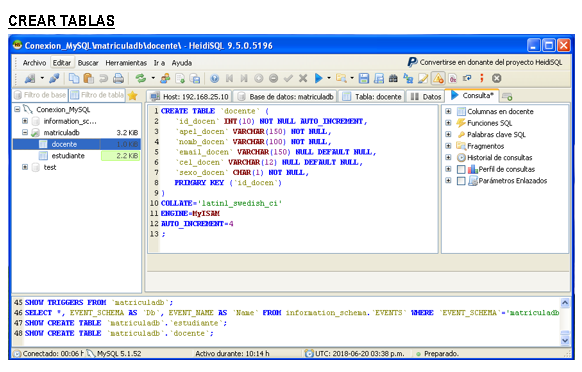
\includegraphics[width=13cm]{./Imagenes/24a}
		\end{center}
\end{itemize} 

\begin{itemize}
	\begin{center}
		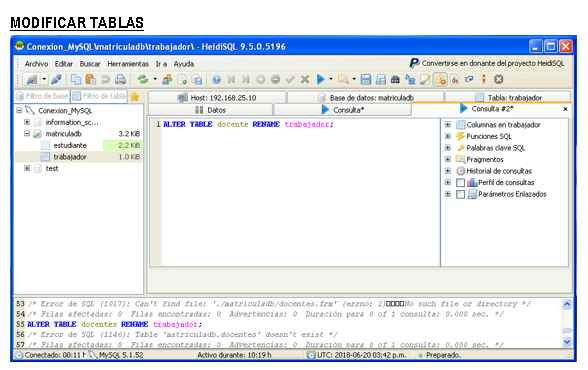
\includegraphics[width=13cm]{./Imagenes/25a}
		\end{center}
\end{itemize} 

\begin{itemize}
	\begin{center}
		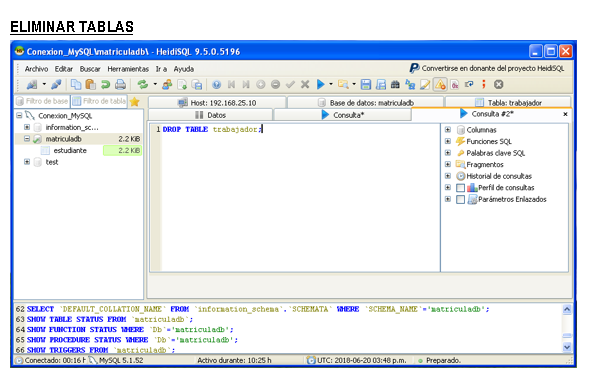
\includegraphics[width=13cm]{./Imagenes/26a}
		\end{center}
\end{itemize} 

\begin{itemize}
	\begin{center}
		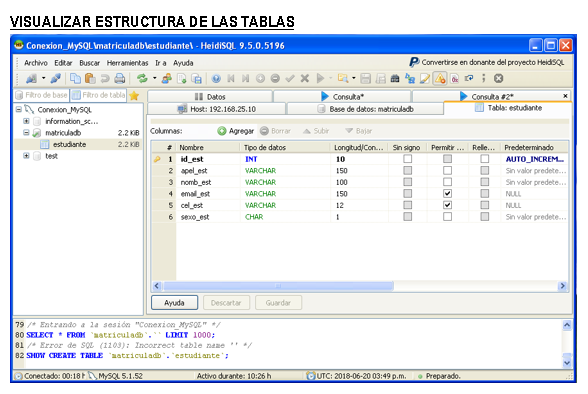
\includegraphics[width=13cm]{./Imagenes/27a}
		\end{center}
\end{itemize} 

\begin{itemize}
	\begin{center}
		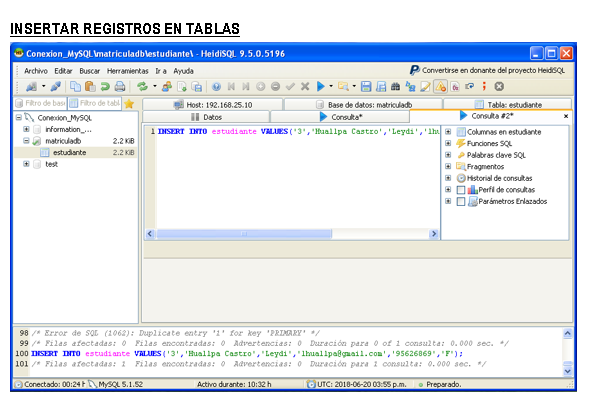
\includegraphics[width=13cm]{./Imagenes/28a}
		\end{center}
\end{itemize} 

\begin{itemize}
	\begin{center}
		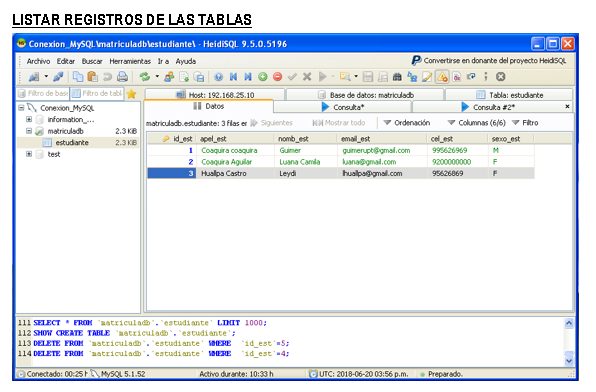
\includegraphics[width=13cm]{./Imagenes/29a}
		\end{center}
\end{itemize} 

\begin{itemize}
	\begin{center}
		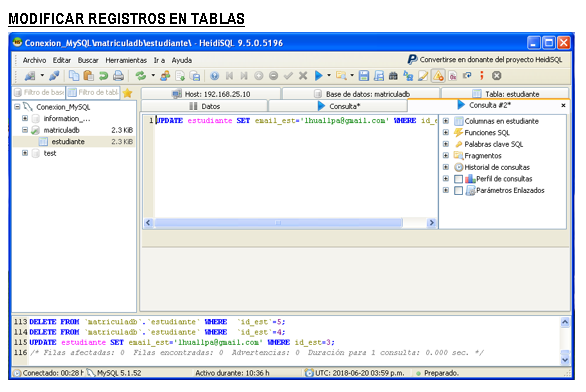
\includegraphics[width=13cm]{./Imagenes/30a}
		\end{center}
\end{itemize} 

\begin{itemize}
	\begin{center}
		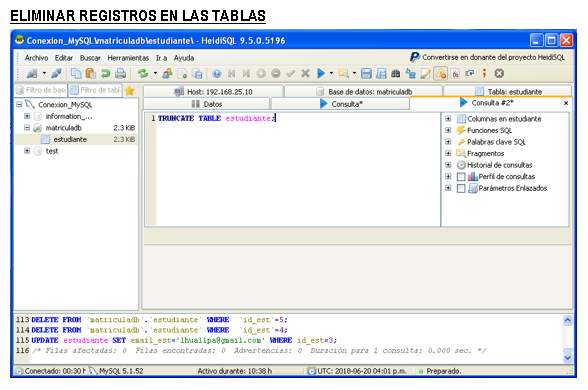
\includegraphics[width=13cm]{./Imagenes/31a}
		\end{center}
\end{itemize} 

\section{Conclusiones} 
\begin{itemize}
	\item  Al finalizar este informe se pueden obtener las siguientes conclusiones:
	\\- El servicio web nos sirve para implementar y administrar nuestras páginas web y sitios web..
\end{itemize}
\\

\section{Recomendaciones} 
\begin{itemize}
	\item  Se recomienda al estudiante y compañeros a practicar constantemente  los diferentes servicios de Linux  y así poder tener una mejor administración en los servicios dentro de una empresa.
\end{itemize}

\section{Bibliografía} 
\begin{itemize}
    \item  https://www.anerbarrena.com/truncate-table-mysql-5051/
\\- https://dev.mysql.com/downloads/mysql/
\\- https://es.wikihow.com/instalar-un-servidor-de-MySQL-en-una-PC
\\- https://es.wikipedia.org/wiki/MySQL
\end{itemize}

